\section{Transformations and Versors}


When applying transformations to our geometric primitives, we want to ensure that
the algebraic structure is preserved. What does this means? Simply that for two
multivectors $A,B$ and a transformation $\mathcal T$ we have that:

\begin{displaymath}
    \mathcal T(A \circ B) = \mathcal T(A) \circ \mathcal T(B).
\end{displaymath}

In the equation above, $\circ$ is any product that can be constructed via the geometric product, for example:

\begin{displaymath}
    \mathcal T(A \wedge B) = \mathcal T(A) \wedge \mathcal T(B),
\end{displaymath}

\begin{displaymath}
    \mathcal T(A \cdot B) = \mathcal T(A) \cdot \mathcal T(B),
\end{displaymath}

\begin{displaymath}
    \mathcal T(A B) = \mathcal T(A) \mathcal T(B),
\end{displaymath}

Now, a $k$-versor $\mathcal V$ is defined by the geometric product of $k$ invertible vectors. This means that
$\mathcal V := v_k ... v_2 v_1$.


\subsection{Reflections}

The reflection around a $\mathbf a$ line can be performed via
\begin{displaymath}
    \mathbf a X \mathbf a^{-1},
\end{displaymath}
where $X$ is a multivector (i.e. it can be a scalar, a vector,a  blade, or a multivector with multiple grades).
We've actually shown this transformation for vectors, but one can apply induction in order to prove
it's validity to any blade, and then, through linearity, show it's validity to any multivector.

We know that a vector $\mathbf a$ is the dual representation of a hyperplane, i.e. if
we consider $\mathbf a$ to be the vector normal to a plane, then any point $\mathbf x$
that falls into this plane satisfies the condition that $\mathbf a \cdot \mathbf x = 0$.
This condition of null inner product is the dual expression. It provides a way of checking
whether a point belongs to the plane, but it does not provide an expression for the actual
points in the plane.

The reflection formula for the hyperplane represented as the dual to $\mathbf a$ is

\begin{displaymath}
    \mathbf a \mathbf{\hat X} \mathbf a^{-1}.
\end{displaymath}

Note that this formula only applies to blade, i.e. $\mathbf X$ is a blade. The reason is clear, the
involution formula is $\mathbf{\hat X} = (-1)^{\text{grade}(\mathbf X)} \mathbf X$, and the grade
operator is only well defined for blades.


\subsection{Rotations}

A rotation cane be constructed from an even number of reflections. Let
$\mathbf a$ and $\mathbf b$ be two vectors with an angle $\phi/2$ from $\mathbf a$ to $\mathbf b$.
Both vectors forma subspace given by $\mathbf a \wedge \mathbf b$. We can then rotate our
vector $\mathbf x$ by an angle $\phi$ by applying the reflection on $\mathbf a$ followed by $\mathbf b$.

\begin{displaymath}
    \mathbf b (\mathbf a \mathbf x \mathbf a^{-1}) \mathbf b^{-1}.
\end{displaymath}

Remember that $\mathbf a^{-1} \mathbf x \mathbf a \mathbf a^{-1}$,
thus

\begin{displaymath}
    \mathbf b  \mathbf a^{-1} \mathbf x \mathbf a \mathbf b^{-1}.
\end{displaymath}

Next, note that:$(\mathbf b / \mathbf a)^{-1} = \mathbf a / \mathbf b$, because

\begin{displaymath}
    (\mathbf b / \mathbf a)(\mathbf a / \mathbf b) = 1 = 
    (\mathbf b / \mathbf a)(\mathbf b / \mathbf a)^{-1}.
\end{displaymath}
and the inverse is unique.

Now, $\mathbf a \mathbf b^{-1} = \frac{\mathbf a \mathbf b}{||\mathbf b||}$



Hence, denoting $R = \mathbf b \mathbf a^{-1}$ we can write the rotation by $R \mathbf x R^{-1}$,
which is again a sandwiching of multivectors.

Note that this transformation is well defined for *any* multivector, and not only vector. Hence:

\begin{displaymath}
    R X R^{-1}
\end{displaymath}
can be used to rotate planes, volumes or some other multivector.

While the reflection transformation depends on the grade of the object to be reflected,
the rotation does not, thus can be applied to any multivector.

\subsection{Projection}

Another important transformation is a projection. Consider two vectors $\mathbf b_1$ and
$\mathbf b_2$. We obtain the subspace defined by them using $\mathbf b_1 \wedge \mathbf b_2 = \mathbf B_{\langle 2\rangle}$.

Now, suppose we want to project a third vector $\mathbf a$ on this subspace. How can we do this?
We could start by applying the left contraction $\rfloor$. Yet, the left contraction
does more than simply project, it also rotates the projected vector. Look the image below (taken from the
book "Álgebra Geométrica e Aplicações" by Fernandes, Lavor and Neto). When we do
$\mathbf a \rfloor \mathbf B_{\langle 2 \rangle} = \mathbf B_{\langle 2\rangle}$, we get the vector $\mathbf c$
in the drawing.

\begin{figure}[H]
    \begin{center}
        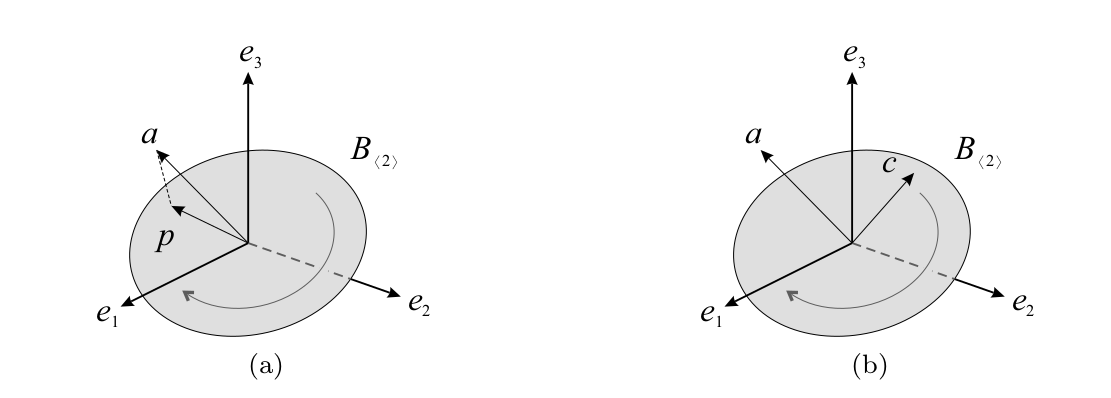
\includegraphics[width=0.85\textwidth]{figures/bladeprojection.png}
    \end{center}
    \caption{Image from \citet{dorst2010geometric} showcasing blade projection.}
    \label{fig:bladeprojection}
\end{figure}

But we want to get $\mathbf p$. How do we do this? We need to apply the left contraction again, but
using it on $c$ with the same subspace but with the inverse rotation. We can do this by using the actual
inverse blade, i.e.

\begin{displaymath}
    \mathbf p = c \rfloor \left(\mathbf B_{\langle 2 \rangle}\right)^{-1}.
\end{displaymath}

Thus, the projection formula becomes:

\begin{displaymath}
    \text{Proj}_{\mathbf B} (\mathbf x) = \left(\mathbf x \rfloor \mathbf B_{\langle 2 \rangle}\right) \rfloor \left(\mathbf B_{\langle 2 \rangle}\right)^{-1}
\end{displaymath}

This formula works fine even for arbitrary blades, **but only in Euclidean spaces**, i.e. spaces with the Euclidean metric.
And we are actually going to work on spaces that are not Euclidean (e.g. Conformal space). So, instead of
this formula for projection, we do:

\begin{displaymath}
    \text{Proj}_{\mathbf B} (\mathbf A) = \left(\mathbf A \rfloor \left(\mathbf B_{\langle 2 \rangle}\right)^{-1}\right) \rfloor \mathbf B_{\langle 2 \rangle},
\end{displaymath}
where $\mathbf A$ is a blade.

First, note that exchanging the order of the inverse does not alter our previous argument of how to obtain the projection. The only
difference is that we start rotating in the other direction. Yet, this other formulation will come in hand when we are in
spaces other than Euclidean, where we'll have multivectors with null norms, which means that they are not invertible. Yet,
we can still do an operation akin to the inverse, and by finishing with the left contraction on $\mathbf B$,
we guarantee that our projected blade will be on the correct subspace.

\subsection{Rotors}

Consider our rotation multivector $R = \mathbf b / \mathbf a$. Depending on the norms
of the vectors, our multivector $R$ will have a norm different than 1. If we normalize it,
we get what is called a **rotor**.

A more precise definition of a rotor is that a
"A rotor R is the geometric product of an even number of unit vectors, such that $R \tilde{R} = 1$" - Leo Dorst
For example, $R = \mathbf b_n \mathbf a_n$, where both are unit vectors, which means that $\mathbf a_n^{-1} = \mathbf a_n$.
Therefore, we have
\begin{displaymath}
    R[X] = R X R^{-1} = (\mathbf b_n \mathbf a_n) X (\mathbf b_n \mathbf a_n)^{-1}  = R X \tilde{R}.
\end{displaymath}

Our multivector is not normalized. We can do this by dividing it by it's norm, or by normalizing the
vectors themselves.
Note that we can construct our rotor by either normalizing the vectors
or the multivector itself.
For normalized vectors, we have $\mathbf b_n /\mathbf a_n = \mathbf b_n \mathbf a_n$.
Remember the formula for the inverse:
\begin{displaymath}
    X^{-1} = \frac{\tilde{X}}{||\mathbf X ||^2}.
\end{displaymath}

Since the norm is equal to 1, we have $X^{-1}= \tilde{X}$.
Thus, for a rotor we have $R \tilde{R} = 1$


Note another important aspect of our rotors. The formula of a rotor can be written as:

\begin{displaymath}
    R = \mathbf b_n \mathbf a_n = \mathbf b_n \cdot \mathbf a_n + \mathbf b_n \wedge \mathbf a_n =
    cos(\phi/2) - \mathbf a_n \wedge \mathbf b_n = 
    cos(\phi/2) - \mathbf I sin(\phi/2),
\end{displaymath}
where
$\mathbf I$ is the unit blade of $\mathbf a_n \wedge \mathbf b_n$, i.e.
\begin{displaymath}
    \mathbf I = \frac{\mathbf a_n \wedge \mathbf b_n}{||\mathbf a_n \wedge \mathbf b_n||},
\end{displaymath}
and $\phi/2$ is the angle between $\mathbf a_n$ and $\mathbf b_n$.

\subsection{Versors}

As we've seen, transformations such as rotations and reflections are done via sandwiching a multivector.
We can generalize these transformations by the fact that they are all comprised of the sandwiching of versors.

\begin{definition}[Versor]
    A k-versor $V$ is any multivector which can be described as the geometric
    product of k non-null vectors, i.e. $V = \mathbf v_k ... \mathbf v_1$, where $\mathbf v_i^{-1}$
    exists for every $i \in \{1,...,k\}$.
\end{definition}

Note that $V X V^{-1} = \mathbf v_k...\mathbf v_1 X (\mathbf v_k...\mathbf v_1)^{-1}$. This is almost the formula
we had for applying multiple reflections. We can rearrange the terms in the right side to obtain:

\begin{displaymath}
    (-1)^k\mathbf v_k...\mathbf v_1  X  \mathbf v_1^{-1}...\mathbf v_k^{-1} =(-1)^k V  X V^{-1}
\end{displaymath}

which is the same as applying the reflection over $\mathbf v_1$ followed by the reflection over $\mathbf v_2$ until $\mathbf v_k$.

Hence, a versor can be **even** or **odd**, where the first is if the number $k$ is even and the latter if the number $k$
is odd. This gives us:
\begin{displaymath}
    V[X] = V X V^{-1} \ \text{ if }V \text{ is even}\\
    V[X] = V \hat{X} V^{-1} \ \text{ if }V \text{ is odd}\\
\end{displaymath}

A very important property of versors is that they preserve the geometric product and all the other operations
that are built from it (e.g. outer prodct, left contraction, right contraction, scalar product).
This is known as the covariance of the versors transformations:
\begin{displaymath}
    V[A B] = V[A]V[B]\\
    V[A \cdot B] = V[A]\cdot V[B]\\
    V[A \wedge B] = V[A]\wedge V[B].
\end{displaymath}

This is easy to show. If $V$ is even, we have:
\begin{displaymath}
    V[A B] = V A B V^{-1} = V A (V^{-1} V) B V^{-1} =(V A V^{-1}) (V B V^{-1}) = V[A] V[B].
\end{displaymath}
If $V$ is odd, we have:
\begin{displaymath}
    V[A B] = V \widehat{A B} V^{-1} = V \hat{A} \hat{B} V^{-1} =V \hat{A} V^{-1} V \hat{B} V^{-1} = V[A] V[B].
\end{displaymath}
We used the fact that $\widehat{A B} = \hat{A} \hat{B}$.
Note that a rotor is also a versor, since $R = \mathbf b_n \mathbf a_n^{-1}$ which are both invertible vectors.

\subsection{Blade Exponentiation}

First, remember that we can write rotor as:
\begin{displaymath}
    R_{\mathbf I \phi/2} = cos(\phi/2) - \mathbf I sin(\phi/2),
\end{displaymath}
where $\mathbf I$ is the normalized subspace for the rotation angle.
From this formula, we can define the rotor as an exponential, i.e.

\begin{displaymath}
    R_{\mathbf I \phi/2} = cos(\phi/2) - \mathbf I sin(\phi/2) = e^{-\mathbf I\phi/2}.
\end{displaymath}

We know how to sum and multiply blades. Thus, we can define it's exponential:

\begin{align}
    &\text{exp}(\mathbf A) = \sum^\infty_{n=0} \frac{\mathbf A^n}{n!} \\
    &\text{ if }\mathbf A^2 =-\alpha^2 \implies \text{exp}(\mathbf a) = cos\alpha + \frac{sin\alpha}{\alpha} \mathbf A \\
    &\text{ if }\mathbf A^2 = 0 \implies \text{exp}(\mathbf a) = 1 + \mathbf A\\
    &\text{ if }\mathbf A^2 =\alpha^2 \implies \text{exp}(\mathbf a) = cosh \alpha + \frac{sinh \alpha}{\alpha}.
\end{align}

